% ==============================================================================
% Secção 5: Qualidade e eficiência da execução
% ==============================================================================

\subsection{Plano de trabalhos e afetação de recursos}
\begin{campotexto}
\instrucao{descrever a estrutura de gestão que pretende adotar, em particular a coordenação entre participantes, os encontros previstos e a estrutura de reporte. O desenvolvimento deste ponto dependerá da dimensão do projeto e, em particular, da existência de participantes de distintas entidades. Prevê-se uma duração máxima de 3 anos para o período financiado. Descrever mecanismos de tomada de decisão e demonstrar a sua adequação à dimensão e complexidade do projeto. Identificar os principais riscos do projeto e planos de contingência propostos. (Máx. 1000 caracteres)}
\end{campotexto}

\subsubsection{Lista de Milestones (designação, data, descrição)}
\begin{campotexto}
\instrucao{Um milestone ou marco é uma data em que se atingiu determinado objetivo ou se completou uma fase. Indique uma lista calendarizada de milestones, com uma periodicidade de cerca de 6 meses a 1 ano, que permita a avaliadores externos aferir se os trabalhos do projeto estão ou não a progredir para os objetivos apontados na candidatura. Preencher uma tabela por milestone, até um máximo de 6. Replicar a tabela consoante necessário.}
\end{campotexto}

% --- Macro auxiliar para tabelas de milestones ---
\newcommand{\tabelaMilestone}[1]{%
  \begin{table}[H]
  \centering\small
  \begin{tabularx}{\textwidth}{L{0.34\textwidth} Y}
    \toprule
    \rowcolor{uatablehead}
    \multicolumn{2}{l}{\sffamily\bfseries\color{uadark} #1} \\
    \midrule
    \sffamily\bfseries Designação do milestone (máx. 60 caracteres) & \\ \arrayrulecolor{uaborder}\hline
    \sffamily\bfseries Data (dd/mm/aaaa) & \\ \hline
    \sffamily\bfseries Descrição (máx. 300 caracteres) & \\
    \arrayrulecolor{black}\bottomrule
  \end{tabularx}
  \end{table}
}

\tabelaMilestone{MILESTONE 1}
\tabelaMilestone{MILESTONE $n$}

\subsubsection{Cronograma}
\begin{campotexto}
\instrucao{Descrever sumariamente a estrutura e lógica de estruturação do plano de trabalhos. Identificar as principais atividades e tarefas previstas em 3.3.6 e as suas relações e dependências. Resumir a calendarização e a associação às diferentes atividades dos milestones descritos em 4.2. Listar os entregáveis associados ao projeto, a sua associação às diferentes atividades e a sua calendarização. Apresentar um diagrama de Gantt com o plano das atividades e tarefas do projeto.}
\end{campotexto}

\begin{table}[H]
\centering\small
\caption{Lista de milestones}
\begin{tabularx}{\textwidth}{L{0.15\textwidth} L{0.15\textwidth} Y L{0.16\textwidth}}
  \toprule
  \rowcolor{uatablehead}
  \sffamily\bfseries\color{uadark} N.º milestone &
  \sffamily\bfseries\color{uadark} N.º da tarefa &
  \sffamily\bfseries\color{uadark} Título &
  \sffamily\bfseries\color{uadark} Data \\
  \midrule
  M1.1 & T1.1 & & \\ \arrayrulecolor{uaborder}\hline
       &      & & \\
  \arrayrulecolor{black}\bottomrule
\end{tabularx}
\end{table}

\begin{table}[H]
\centering\small
\caption{Lista de entregáveis (resultado sob a forma de publicação ou outro tipo de elemento que permita contextualizar, avaliar ou aferir o resultado alcançado)}
\begin{tabularx}{\textwidth}{L{0.14\textwidth} L{0.12\textwidth} Y L{0.13\textwidth} L{0.26\textwidth}}
  \toprule
  \rowcolor{uatablehead}
  \sffamily\bfseries\color{uadark} N.º entregável &
  \sffamily\bfseries\color{uadark} N.º tarefa &
  \sffamily\bfseries\color{uadark} Título &
  \sffamily\bfseries\color{uadark} Data &
  \sffamily\bfseries\color{uadark} Tipo \\
  \midrule
  E1.1 & T1.1 & & & \instrucao{(Documento; Relatório; Protótipo; Demonstrador; Piloto; Website; Publicação; etc.)} \\ \arrayrulecolor{uaborder}\hline
       &      & & & \\
  \arrayrulecolor{black}\bottomrule
\end{tabularx}
\end{table}

\begin{figure}[H]
  \centering
  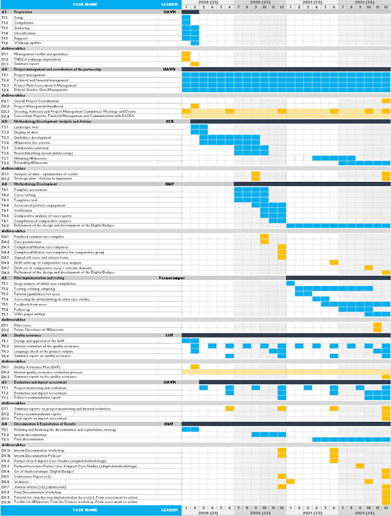
\includegraphics[width=0.72\textwidth]{g.png}
  \caption{Mapa de Gantt (ilustrativo).}
\end{figure}

\subsection{Qualidade da equipa (e do consórcio)}
\begin{campotexto}
\instrucao{Máx. 1000 caracteres}
\end{campotexto}
